%%%%%%%%%%%%%%%%%%%%%%%%%%%%%%%%%%%%%%%%%%%%%%%%%%%%%%%%
% IE643 Course Project Poster (based on the given template)
% Content = the "classic" adapter (configs/ltx2b_classic.yaml). Page geometry, fonts, frames unchanged.
%%%%%%%%%%%%%%%%%%%%%%%%%%%%%%%%%%%%%%%%%%%%%%%%%%%%%%%%
\documentclass[a0,portrait]{a0poster}
\usepackage[top=5cm, bottom=0.3cm, left=5cm, right=3cm]{geometry}
\usepackage[compact]{titlesec}
\usepackage{multicol}
\columnsep=100pt
\columnseprule=15pt
\usepackage[svgnames]{xcolor}
\usepackage{palatino}
\usepackage{xkeyval}
\usepackage{graphicx}
\setlength{\abovecaptionskip}{5pt plus 5pt minus 3pt}
\graphicspath{{figures/}}
\usepackage{booktabs}
\usepackage[font=small,labelfont=bf]{caption}
\usepackage{amsfonts, amsmath, amsthm, amssymb}
\usepackage{csquotes}
\usepackage{wrapfig}
\usepackage{multirow}
\usepackage{makecell}
\def\columnseprulecolor{\color{NavyBlue}}%
\usepackage{framed}
\colorlet{frameborder}{NavyBlue}
\begin{document}
%------------------------------ HEADER ------------------------------
\begin{minipage}[c]{\linewidth}
\vspace{0.1cm}
\noindent\makebox[\textwidth][c]{
\begin{minipage}[c]{0.14\linewidth}
\vspace{0pt}\raggedright
\hspace{1cm}

\includegraphics[scale=1.3,width=\linewidth]{figures/logo.png}
\end{minipage}
\hfill
\begin{minipage}[c]{0.75\textwidth}
\centering
\Huge \color{Green} \textbf{IE643 Course Project}\\[0.5cm]
\Huge \color{NavyBlue} \textbf{Trajectory-Conditioned Motion-Control Adapter for Image-to-Video Diffusion}\\[0.5cm]
\Large \color{NavyBlue} \textbf{VIBE}\\[0.5cm]
\large \color{Black} \textbf{Mithra Bijumon $^{1}$ (24b0040), Stuti Mahajan $^{2}$ (24b0067)}\\[0.2cm]
\small \text{24b0040@iitb.ac.in$^{1}$, 24b0067@iitb.ac.in$^{2}$}\\
\large \color{Green} \textbf{}\\
\end{minipage}
\begin{minipage}[c]{0.145\textwidth}
\vspace{0pt}\raggedleft

\includegraphics[scale=1.3,width=\linewidth]{figures/IE643-Logo.pdf}
\hspace{1cm}
\end{minipage}}
\\[0.1cm]
%----------------------------------------------------------------------------------------
\color{NavyBlue}\setlength\FrameRule{25pt}
\begin{framed}
\vspace{0.5cm}
\begin{multicols}{2}
\color{Black}
%------------------------------ ABSTRACT ------------------------------
\section*{Abstract}
We give a model one image and one drawn path, and want a video where a single object follows that path. We keep LTX-Video 2B frozen and train only a small ControlNet-style adapter (5.9M parameters). The adapter writes into the frozen model only around the object, so the background is left alone. A focus loss trains object and background separately, and our metrics score them separately too.

%------------------------------ INTRODUCTION ------------------------------
\section*{Introduction}
\begin{itemize}
    \item \textbf{Task:} image + drawn path $\rightarrow$ generated video where the object moves along the path.
    \item \textbf{Why it matters:} video models make realistic clips but give little control over where the object goes; this control is useful for animation, film previsualisation and simulation.
    \item Deep learning lets us learn this control from data, without retraining the huge base model.
    \item Instructor feedback on our earlier version: background moved with the object, results changed a lot with the seed, forward and backward paths behaved differently, out-of-domain images were poor.
\end{itemize}
\vspace{0.4cm}
\begin{center}
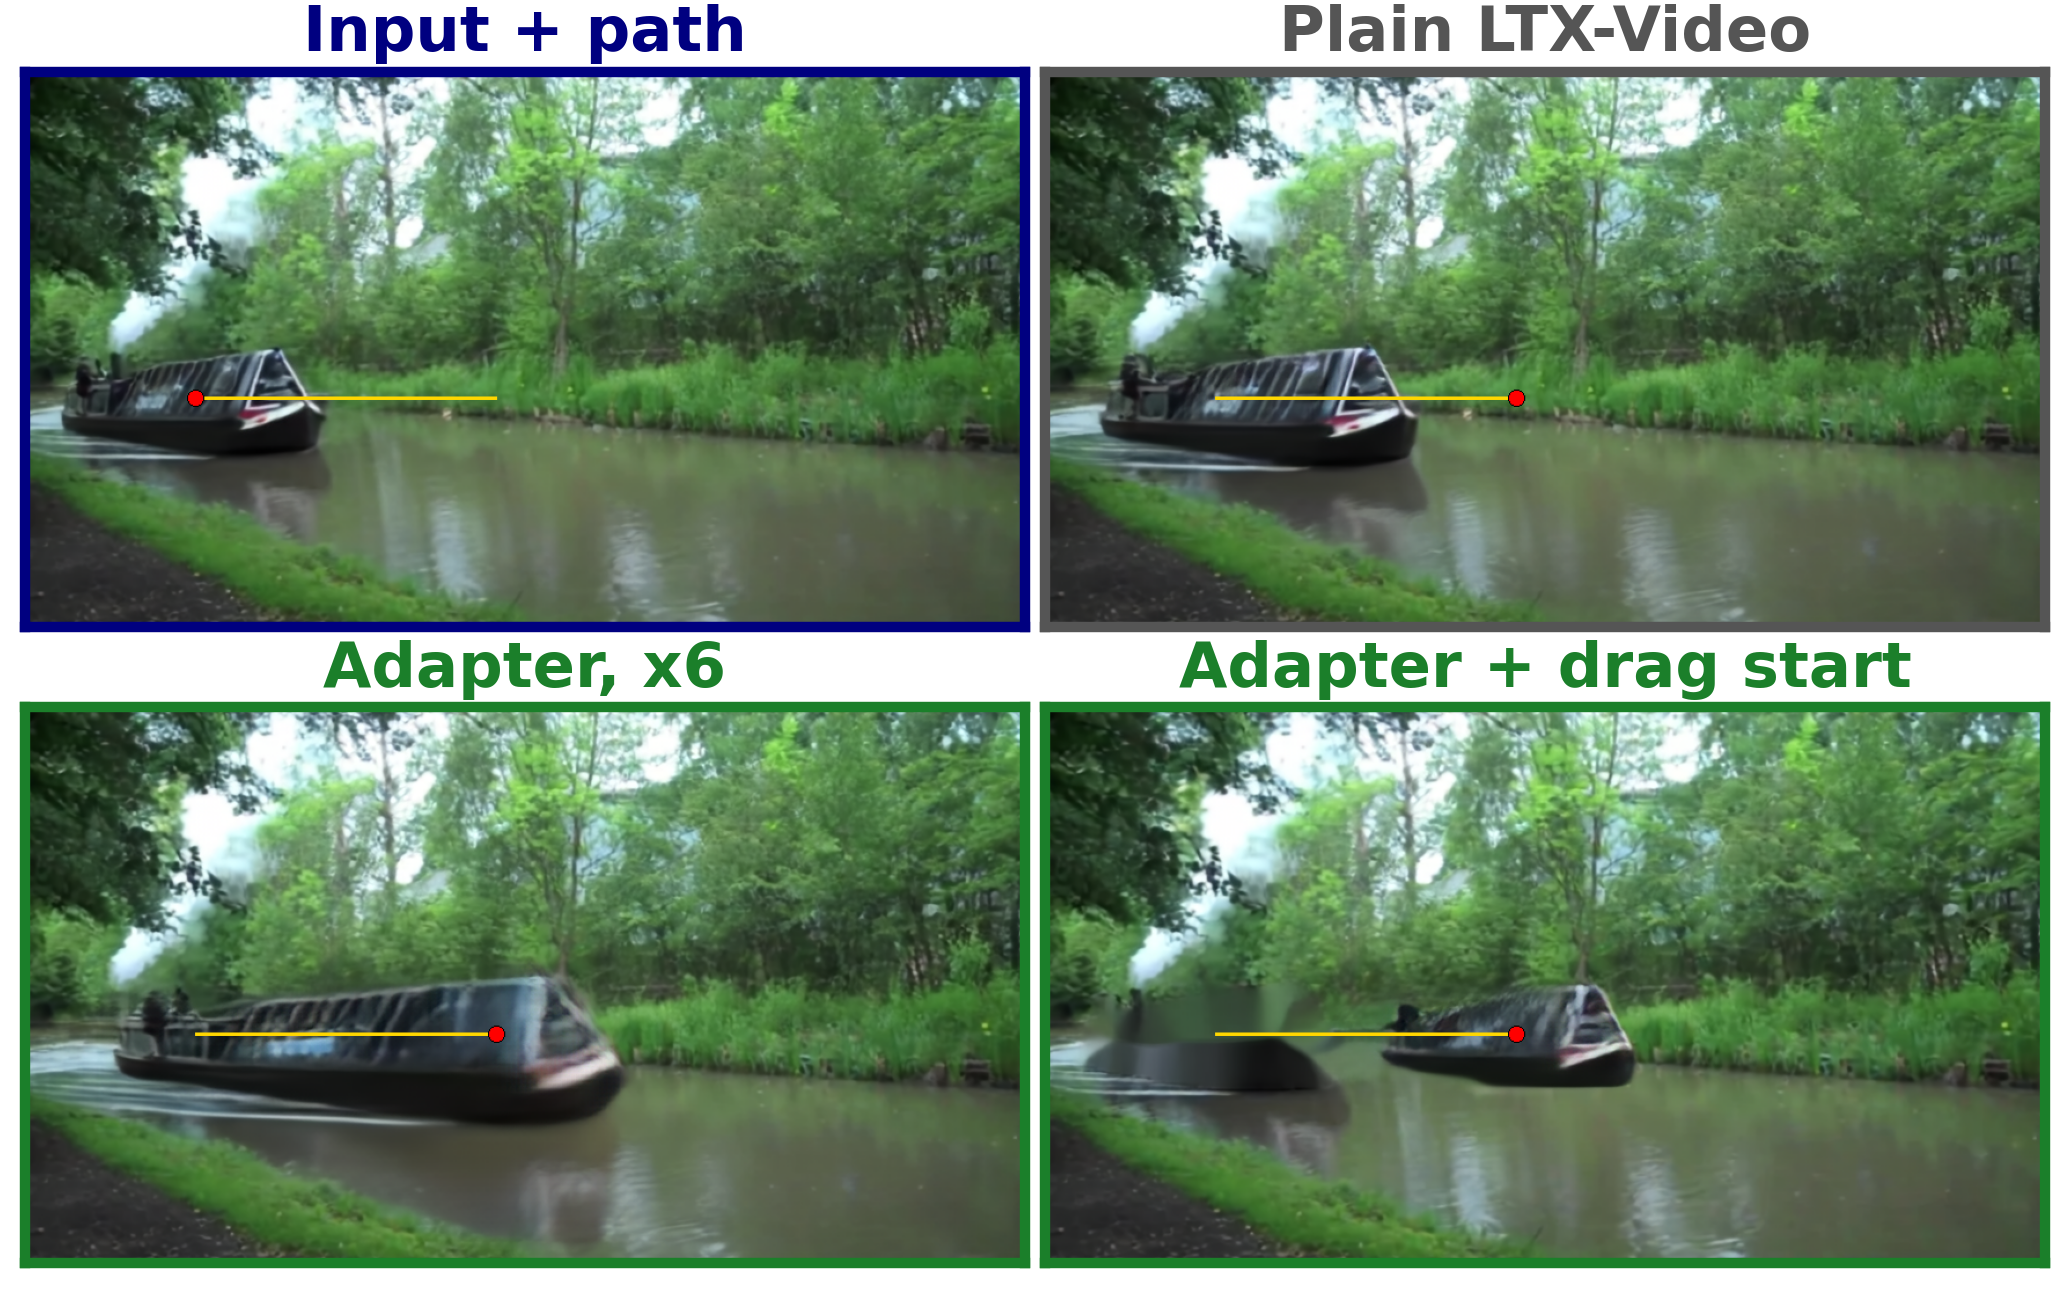
\includegraphics[width=0.5\linewidth,height=11cm,keepaspectratio]{figures/Intro.png}
\captionof{figure}{\color{Blue}Input image and path, and the last frame of plain LTX-Video, our adapter (strength $\times$6) and the adapter with a drag-video start}
\label{Intro}
\end{center}
We outline our major \textbf{contributions} below:
\vspace{-\baselineskip}\\
\begin{itemize}
    \item Small adapter on a \textbf{frozen} LTX-Video (no LoRA), injected only around the object.
    \item \textbf{Focus loss:} object and background tokens trained separately.
    \item Inference dials: adapter \textbf{strength}, motion guidance, optional drag-video start.
    \item Metrics that score \textbf{object and background motion separately}.
\end{itemize}

%------------------------------ WORKFLOW ------------------------------
\section*{Workflow}
Figure \ref{workflow} shows our workflow: data and labels, condition, adapter training, generation, then evaluation.
\begin{center}
    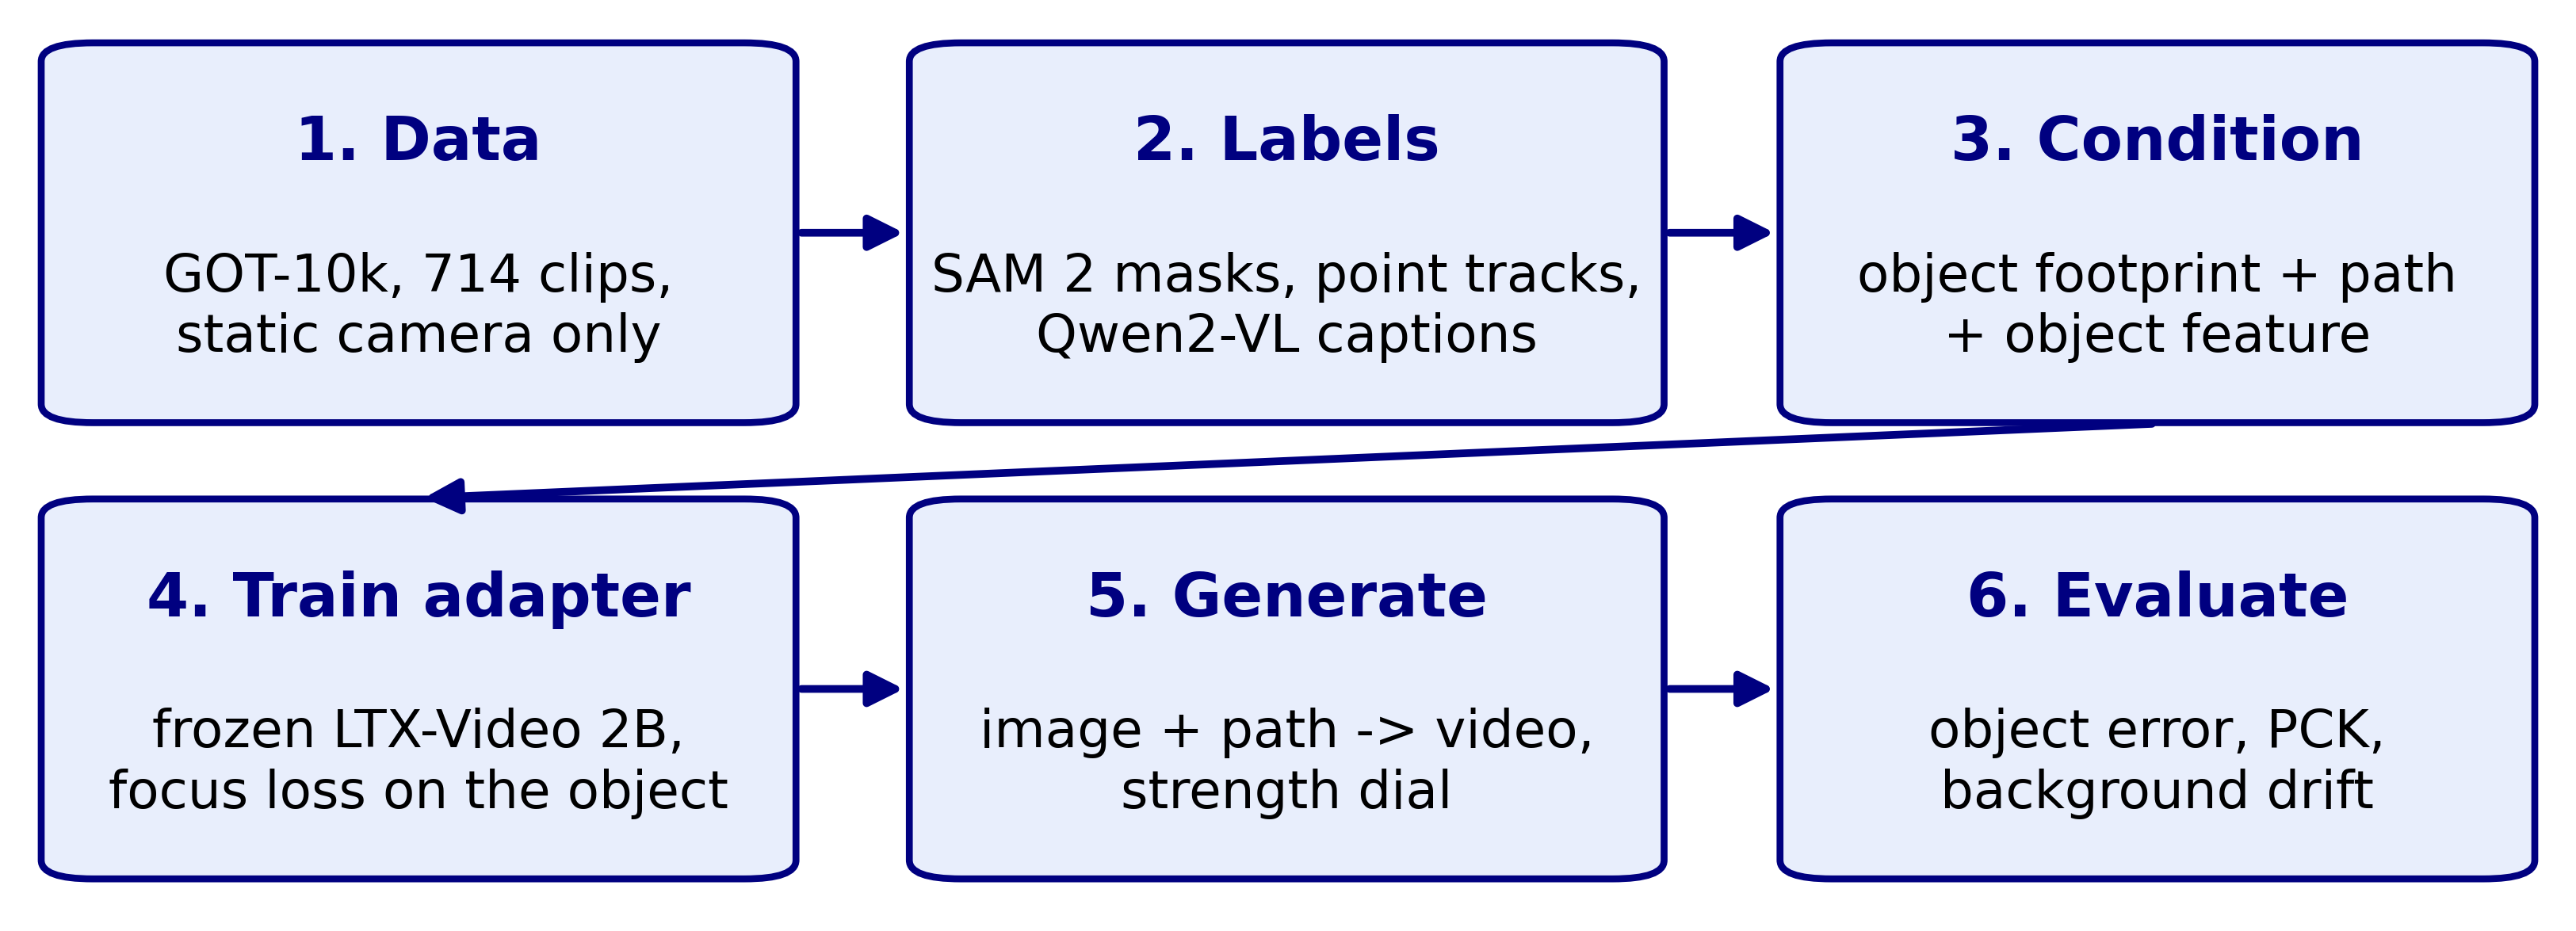
\includegraphics[width=0.95\linewidth,height=12cm,keepaspectratio]{figures/Workflow.png}
    \captionof{figure}{\color{Blue} Overall Workflow}
    \label{workflow}
\end{center}

%------------------------------ METHODOLOGY ------------------------------
\section*{Methodology}
Figure \ref{Arch} shows the architecture.
\begin{center}
    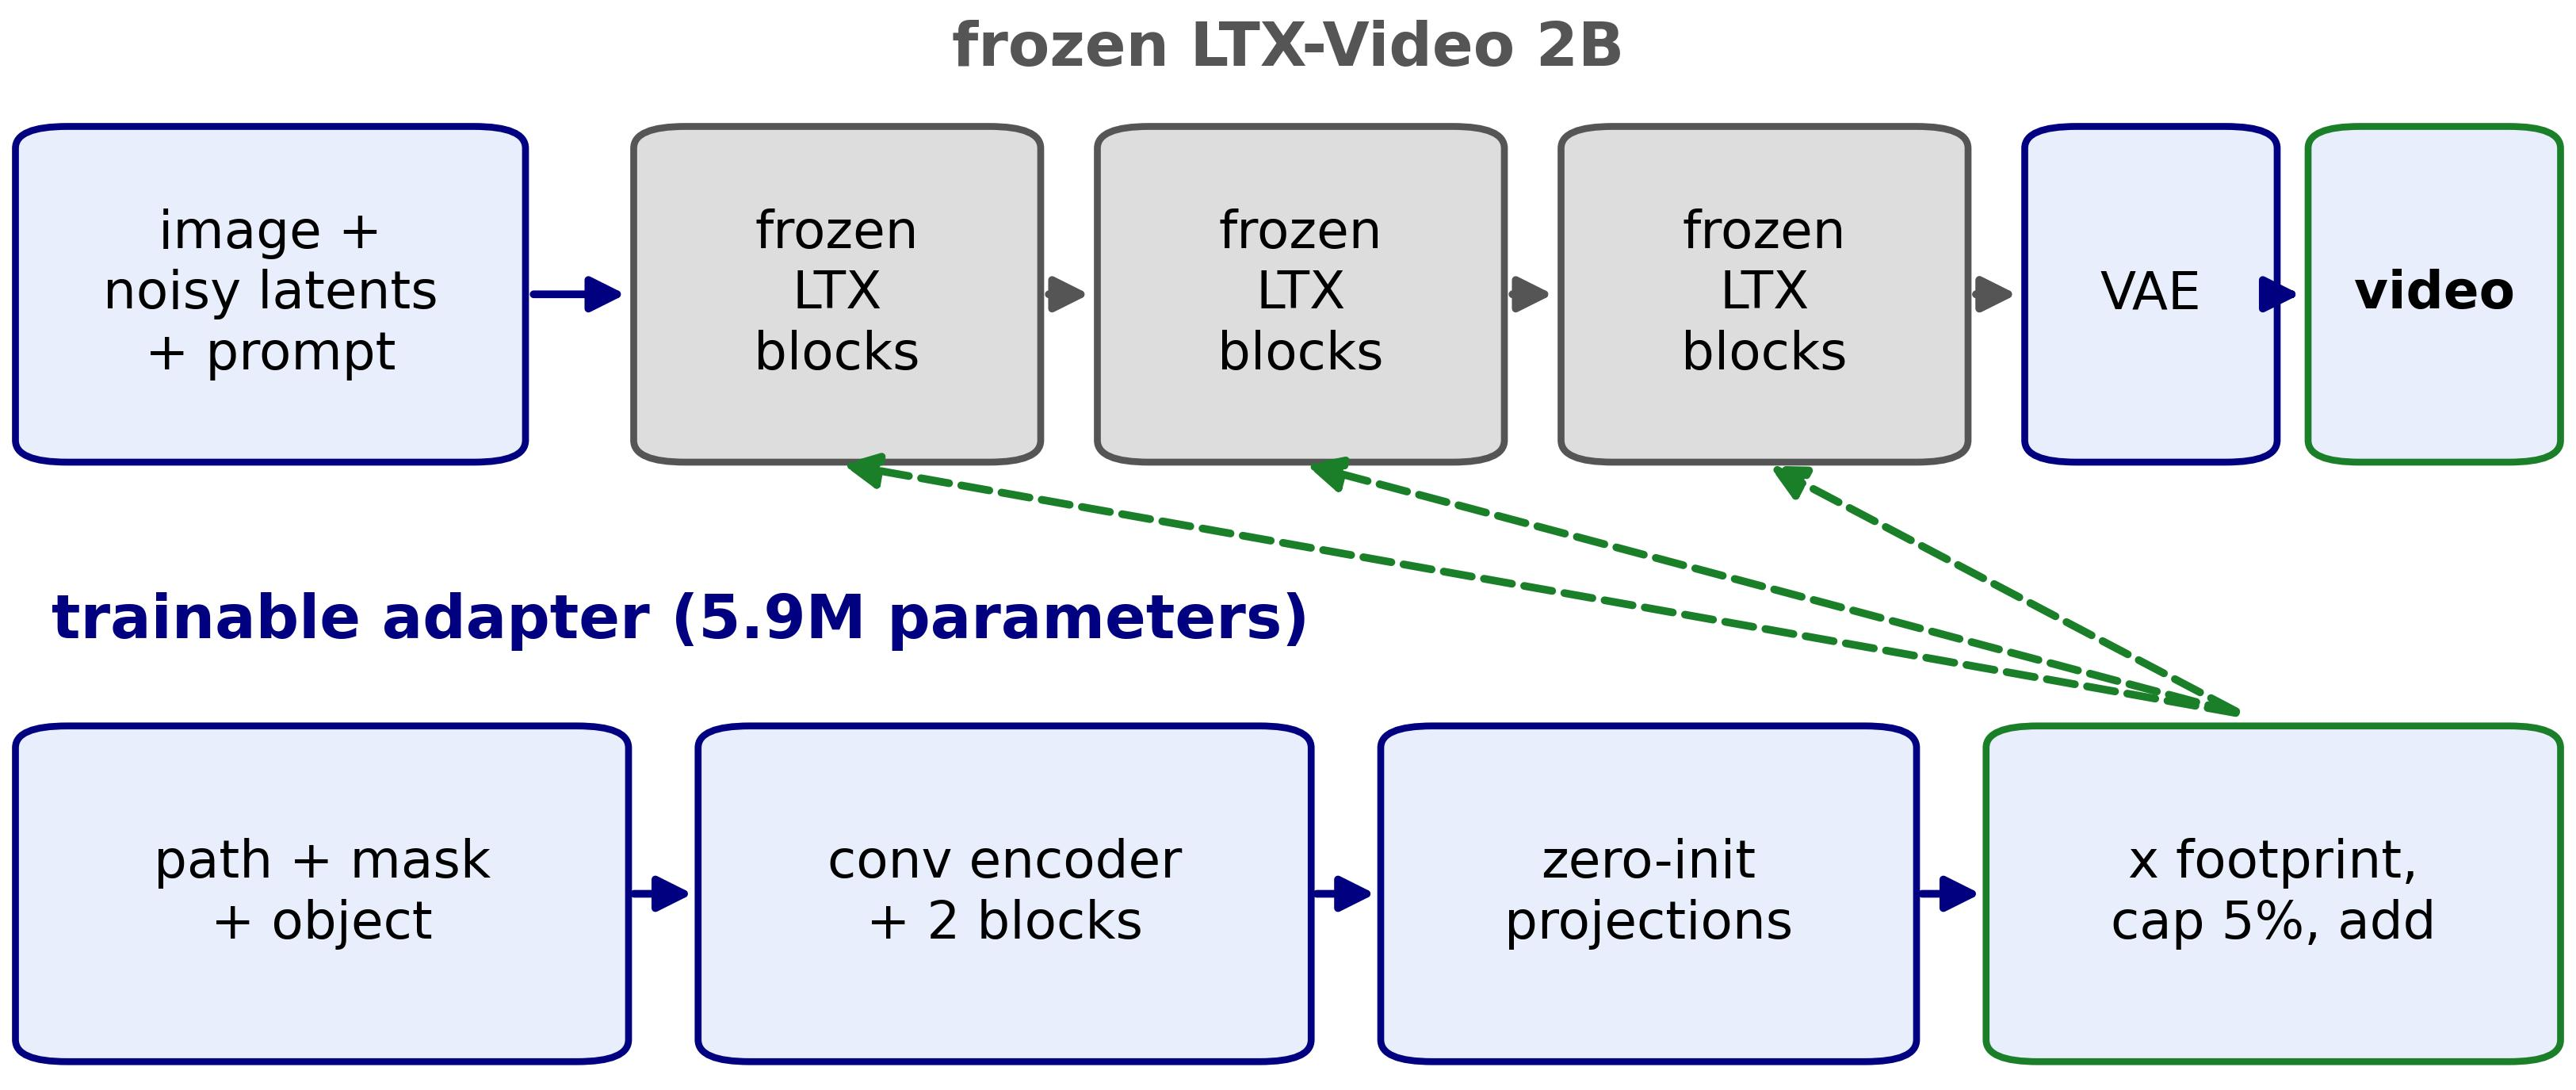
\includegraphics[width=0.95\linewidth,height=14cm,keepaspectratio]{figures/Deep-Neural-Network-Model.jpg}
    \captionof{figure}{\color{Blue} Overall Architecture}
    \label{Arch}
\end{center}
\begin{itemize}
    \item \textbf{Condition:} the object's SAM silhouette moved along the path, its displacement, and the object's own feature, drawn on the video latent grid.
    \item \textbf{Adapter:} conv encoder + 2 transformer blocks, then zero-initialised linear projections added after every 2nd frozen LTX block (forward hooks). Training starts from the base model.
    \item \textbf{Object-only injection:} residual $\times$ Gaussian footprint (radius 2$\times$ the object), scaled by the hidden state's RMS and capped at 5\%.
    \item \textbf{Focus loss:} object and background tokens averaged separately (SAM 2 masks), object weight 5, later frames weighted more.
    \item \textbf{Per-clip prompts:} Qwen2-VL-2B caption for each clip.
    \item \textbf{Training:} 10 epochs, batch 1, lr $3\times10^{-5}$ with cosine decay; condition dropped for 10\% of samples.
    \item \textbf{At inference:} adapter strength ($\times$1 to $\times$6) and motion guidance; optionally start from a noised ``drag video'' (object cut out, moved along the path).
\end{itemize}

%------------------------------ DATASET ------------------------------
\section*{Dataset Details}
\begin{center}
\scalebox{1.1}{
\begin{tabular}{|l|l|}
\hline
\textbf{Property} & \textbf{Value} \\
\hline
Source & GOT-10k \\
Clips used & 714 single-object clips \\
Filtering & moving-camera clips removed \\
Object masks & SAM (first frame), SAM 2 (all frames) \\
Captions & Qwen2-VL-2B, one per clip \\
Test paths & left, right, up, down (fwd and bwd) \\
Extra test set & clean out-of-domain images \\
\hline
\end{tabular}}
\end{center}

%------------------------------ NOVELTY ------------------------------
\section*{Novelty Assessment}
We designed one experiment per point of instructor feedback:
\begin{center}
\scalebox{1.0}{
\begin{tabular}{|p{0.3\linewidth}|p{0.55\linewidth}|}
\hline
\textbf{Problem} & \textbf{What we tried} \\
\hline
Background moves & Object-only injection, separate focus loss \\
\hline
Seed sensitivity & Matched seeds, mean $\pm$ std; fixed unseeded VAE bug \\
\hline
Fwd $\neq$ bwd & Test both directions on same clips \\
\hline
Poor out-of-domain & Separate clean out-of-domain group \\
\hline
Effect too weak & Strength dial and motion guidance at inference \\
\hline
\end{tabular}}
\end{center}
Main test: \textbf{focus loss ON vs OFF} with same seeds, fwd and bwd paths, object error and background motion reported separately (see report).

%------------------------------ RESULTS ------------------------------
\section*{Results}
Object: \texttt{obj\_ate}, \texttt{obj\_dir\_cos}, \texttt{pck@10}. Background: \texttt{bg\_drift}, \texttt{bg\_flow}. 8 clips $\times$ 5 paths, 1 seed, adapter strength $\times$3.
\begin{center}
    \scalebox{1.0}{
        \begin{tabular}{|c|c|c|c|c|c|}
            \hline
            Methods & obj\_ate $\downarrow$ & obj\_dir\_cos $\uparrow$ & pck@10 $\uparrow$ & bg\_drift $\downarrow$ & bg\_flow $\downarrow$ \\
            \hline
            Plain LTX-Video & 0.155 & 0.096 & 0.337 & 0.062 & 0.003 \\
            \textbf{Adapter (Ours)} & \textbf{0.140} & \textbf{0.195} & \textbf{0.400} & \textbf{0.059} & \textbf{0.003} \\
            \hline
        \end{tabular}}\\
    \captionof{table}{\color{Blue} Benchmark: plain LTX-Video vs our adapter (same images, paths, seed)}
    \label{table}
    \vspace{-0.25in}
\end{center}
\vspace{0.25in}
Table \ref{table} compares the two. Findings:
\begin{itemize}
    \item \textbf{The adapter follows the path better:} object error 0.155 $\rightarrow$ 0.140, direction 0.10 $\rightarrow$ 0.20, PCK@10 0.34 $\rightarrow$ 0.40, progress 0.03 $\rightarrow$ 0.10.
    \item \textbf{The background is untouched:} bg\_flow equal, bg\_drift 0.062 $\rightarrow$ 0.059; image quality is unchanged (CLIP similarity 0.943 for both).
    \item \textbf{Forward and backward differ:} right and diagonal improve (direction 0.16 $\rightarrow$ 0.35, 0.48 $\rightarrow$ 0.59); left does not (-0.16), up stays wrong-signed (-0.52 $\rightarrow$ -0.32).
    \item On normal validation clips the loss gain stays $\approx 0$ (best $+0.01\times10^{-3}$ at epoch 4), so the effect shows only when the adapter is amplified; at $\times$6 the boat is stretched (Fig.~\ref{Intro}).
    \item Small test: 8 clips, 1 seed, no out-of-domain images yet. The drag-video start leaves a faint ghost.
\end{itemize}
\IfFileExists{figures/qualitative.png}{%
\begin{center}
    \includegraphics[width=0.95\linewidth,height=10cm,keepaspectratio]{figures/qualitative.png}
    \captionof{figure}{\color{Blue} Qualitative results}
\end{center}}{}

%------------------------------ CONCLUSION ------------------------------
\section*{Conclusion}
\begin{itemize}
    \item A 5.9M-parameter adapter on a frozen LTX-Video trains stably and leaves the background alone.
    \item At strength $\times$3 it follows the path better than plain LTX (object error 0.155 $\rightarrow$ 0.140, PCK@10 0.34 $\rightarrow$ 0.40) without moving the background; the effect is modest and not yet reliable (left and up paths).
    \item Separate object and background metrics make failures easy to see.
    \item \textbf{Future work:} higher learning rate and stronger focus loss, focus ON/OFF and out-of-domain tests, fix partial masks.
\end{itemize}

%------------------------------ REFERENCES ------------------------------
\begin{thebibliography}{6}
\small
\bibitem{ltx} Yoav HaCohen et al. LTX-Video: Realtime Video Latent Diffusion, arXiv, 2024. https://arxiv.org/abs/2501.00103
\bibitem{cnet} Lvmin Zhang, Anyi Rao and Maneesh Agrawala. Adding Conditional Control to Text-to-Image Diffusion Models, ICCV, 2023. https://arxiv.org/abs/2302.05543
\bibitem{sam2} Nikhila Ravi et al. SAM 2: Segment Anything in Images and Videos, arXiv, 2024. https://arxiv.org/abs/2408.00714
\bibitem{cot3} Nikita Karaev et al. CoTracker3: Simpler and Better Point Tracking by Pseudo-Labelling Real Videos, arXiv, 2024. https://arxiv.org/abs/2410.11831
\bibitem{got} Lianghua Huang, Xin Zhao and Kaiqi Huang. GOT-10k: A Large High-Diversity Benchmark for Generic Object Tracking in the Wild, IEEE TPAMI, 2019. https://arxiv.org/abs/1810.11981
\bibitem{qwen} Peng Wang et al. Qwen2-VL: Enhancing Vision-Language Model's Perception of the World at Any Resolution, arXiv, 2024. https://arxiv.org/abs/2409.12191
\bibitem{sdedit} Chenlin Meng et al. SDEdit: Guided Image Synthesis and Editing with Stochastic Differential Equations, ICLR, 2022. https://arxiv.org/abs/2108.01073
\end{thebibliography}

%------------------------------ ACKNOWLEDGEMENTS ------------------------------
\section*{Acknowledgments}
\small \textnormal{We thank the professor and TAs for their feedbacks and guidance.}

\section*{Github Link and Demo Video Link}
\vspace{-0.5cm}
\begin{center}
        \begin{minipage}{0.4\linewidth}
            \centering
            \textbf{Github Repository}\\[1ex]
            
\includegraphics[width=0.5\linewidth]{github_qr.png}
        \end{minipage}\hfill
        \begin{minipage}{0.4\linewidth}
            \centering
            \textbf{Demo Video Link}\\[1ex]
            
\includegraphics[width=0.5\linewidth]{demo_video_qr.png}
        \end{minipage}
\end{center}

\end{multicols}
\vspace{0.5cm}
\end{framed}
\end{minipage}
\end{document}
